\subsubsection{Presentazione dei risultati di ricerca}
Mi riferisco alla presentazione dei risultati della funzionalità di ricerca
\quotes{Browser Top Sites}; la presentazione dei risultati del Box Testuale
discusso in precedenza è analoga a quella descritta in \ref{overview}.
\begin{figure}[ht]
\centering
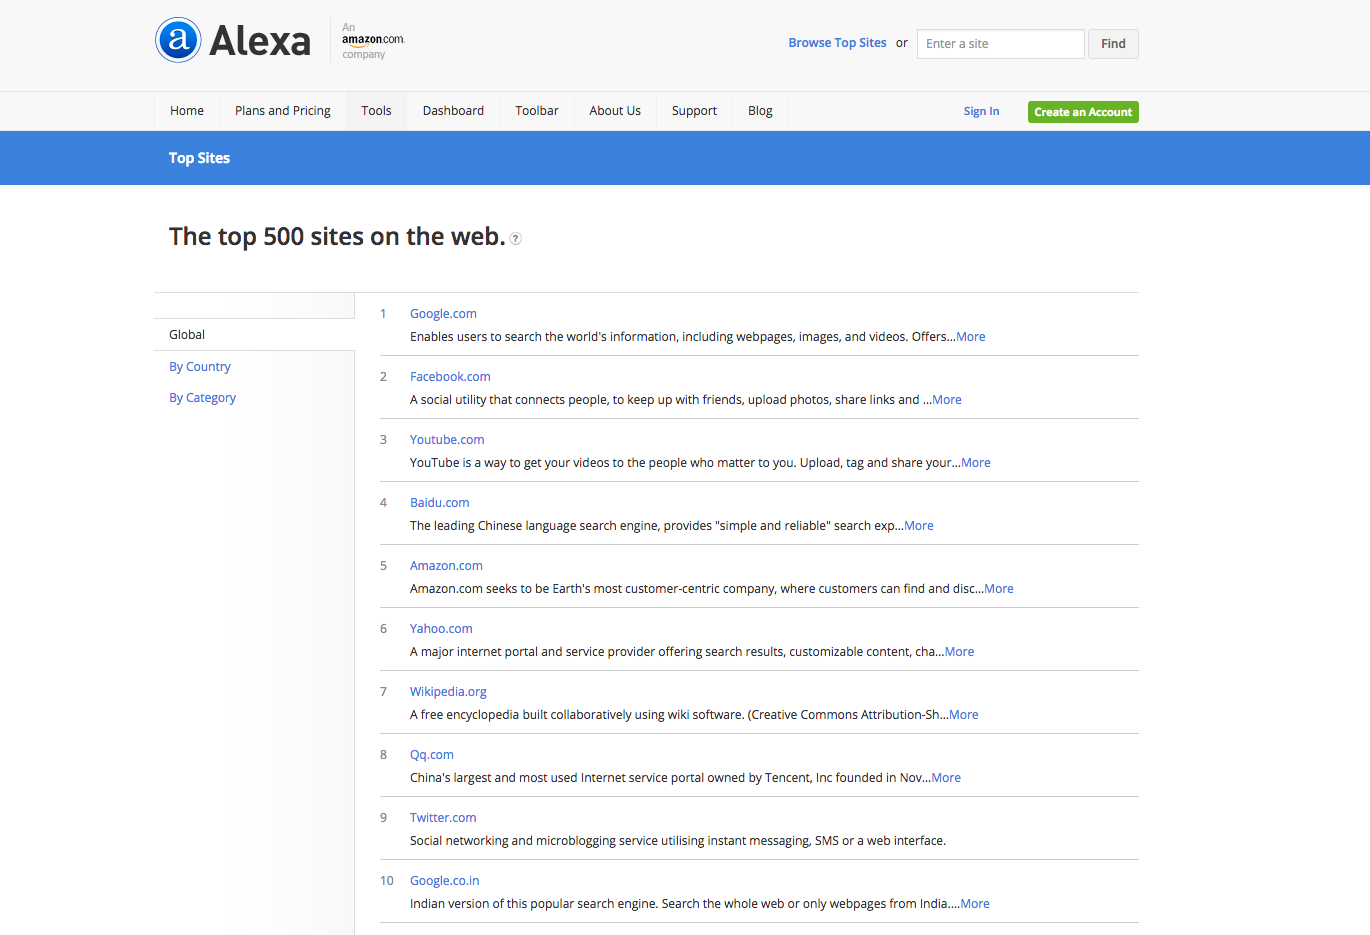
\includegraphics[scale=0.30,keepaspectratio]{{figure/4/searchResult0}.png}
\caption{Risultati di ricerca - Top Sites}
\end{figure}
\FloatBarrier
Ottima la presentazione dei risultati di ricerca: viene utilizzata una lista
numerata con un titolo ed una breve descrizione che si può facilmente espandere,
sulla colonna di sinistra sono indicati i filtri da utilizzare per visualizzare
i risultati. Nel bottom della pagina si possono selezionare i risultati
successivi alla prima pagina.\\
Risultato : \textbf{10}
